%% Final derivation- and positioning-enhanced information-access paper for ICAIF 2026.
%% Compile: latexmk -pdf -interaction=nonstopmode main.tex
\documentclass[sigconf]{acmart}

\settopmatter{authorsperrow=4}
\AtBeginDocument{\providecommand\BibTeX{{\normalfont B\kern-0.5em{\scshape i\kern-0.25em b\kern-0.8em\TeX}}}}
% ACM publication metadata (CC BY-NC-ND).
\setcopyright{cc}
\setcctype{by-nc-nd}
\acmConference[ICAIF '26]{7th ACM International Conference on AI in Finance}{November 14--17, 2026}{Milan, AA, Italy}
\acmBooktitle{7th ACM International Conference on AI in Finance (ICAIF '26), November 14--17, 2026, Milan, AA, Italy}
\acmYear{2026}
\copyrightyear{2026}
\acmDOI{10.1145/3858063.3858812}
\acmISBN{979-8-4007-3087-0/2026/11}

\usepackage{amsmath}
\usepackage{array}
\usepackage{booktabs}
\usepackage{stfloats}
\usepackage{enumitem}
\usepackage{float}
\usepackage{xurl}
\usepackage{graphicx}
\usepackage{placeins}
\setcounter{dbltopnumber}{1}
\renewcommand{\dbltopfraction}{0.82}
\renewcommand{\dblfloatpagefraction}{0.90}
\setlength{\intextsep}{6pt plus 1pt minus 1pt}
\setlength{\textfloatsep}{8pt plus 1pt minus 1pt}
\captionsetup{justification=raggedright,singlelinecheck=false}
\newcommand{\tabnote}[1]{\par\vspace{2pt}\noindent\begin{minipage}{\linewidth}\footnotesize\emph{Note:} #1\end{minipage}}
\emergencystretch=1.2em
\vfuzz=2pt
\setlength{\bibsep}{0pt plus 0.2ex}
% A root-level Overleaf entry qualifies the bibliography's subfolder.
\providecommand{\ReviewBibliography}{refs}

% Generated by src/icaif_v4_assets.py; do not edit.
\newcommand{\SharedKTwo}{1.45}
\newcommand{\SharedKFour}{1.83}
\newcommand{\SharedKSeven}{2.05}
\newcommand{\SharedOverlap}{0.618}
\newcommand{\SharedGross}{0.790}
\newcommand{\SharedOrder}{1.871}
\newcommand{\SharedCommonBeta}{0.725}
\newcommand{\MixedKTwo}{1.67}
\newcommand{\MixedKFour}{2.80}
\newcommand{\MixedKSeven}{3.98}
\newcommand{\MixedOverlap}{0.381}
\newcommand{\MixedGross}{0.457}
\newcommand{\MixedOrder}{0.818}
\newcommand{\MixedCommonBeta}{0.215}
\newcommand{\CoherentKTwo}{1.83}
\newcommand{\CoherentKFour}{3.07}
\newcommand{\CoherentKSeven}{3.89}
\newcommand{\CoherentOverlap}{0.354}
\newcommand{\CoherentGross}{0.413}
\newcommand{\CoherentOrder}{0.662}
\newcommand{\CoherentCommonBeta}{0.147}
\newcommand{\MixedSharedNeff}{+1.93}
\newcommand{\MixedSharedNeffCI}{[+1.76, +2.09]}
\newcommand{\MixedSharedOverlap}{-0.237}
\newcommand{\MixedSharedOverlapCI}{[-0.254, -0.219]}
\newcommand{\MixedSharedGross}{-0.333}
\newcommand{\MixedSharedGrossCI}{[-0.364, -0.306]}
\newcommand{\MixedSharedOrder}{-1.053}
\newcommand{\MixedSharedOrderCI}{[-1.133, -0.992]}
\newcommand{\CoherentSharedNeff}{+1.84}
\newcommand{\CoherentSharedNeffCI}{[+1.58, +2.04]}
\newcommand{\CoherentSharedOverlap}{-0.264}
\newcommand{\CoherentSharedOverlapCI}{[-0.285, -0.239]}
\newcommand{\CoherentSharedGross}{-0.376}
\newcommand{\CoherentSharedGrossCI}{[-0.402, -0.354]}
\newcommand{\CoherentSharedOrder}{-1.209}
\newcommand{\CoherentSharedOrderCI}{[-1.297, -1.128]}
\newcommand{\CoherentMixedNeff}{-0.09}
\newcommand{\CoherentMixedNeffCI}{[-0.28, +0.07]}
\newcommand{\CoherentMixedOverlap}{-0.027}
\newcommand{\CoherentMixedOverlapCI}{[-0.037, -0.015]}
\newcommand{\CoherentMixedGross}{-0.043}
\newcommand{\CoherentMixedGrossCI}{[-0.068, -0.018]}
\newcommand{\CoherentMixedOrder}{-0.156}
\newcommand{\CoherentMixedOrderCI}{[-0.228, -0.086]}
\newcommand{\NullKSeven}{4.83}
\newcommand{\NullKSevenLow}{3.99}
\newcommand{\NullKSevenHigh}{5.60}
\newcommand{\AnalyticNullKSeven}{4.79}
\newcommand{\SharedKappa}{0.437}
\newcommand{\MixedKappa}{0.133}
\newcommand{\CoherentKappa}{0.138}
\newcommand{\NullKappa}{0.077}
\newcommand{\SharedNullShare}{42.5\%}
\newcommand{\MixedNullShare}{82.4\%}
\newcommand{\CoherentNullShare}{80.6\%}
\newcommand{\SharedFirstMarginal}{0.45}
\newcommand{\SharedLastMarginal}{0.05}
\newcommand{\MixedLastMarginal}{0.41}
\newcommand{\CoherentLastMarginal}{0.20}
\newcommand{\SharedNeffRange}{1.34--3.31}
\newcommand{\MixedNeffRange}{2.58--4.59}
\newcommand{\CoherentNeffRange}{3.34--4.38}
\newcommand{\OverlapReductionPercent}{43\%}
\newcommand{\MixedCapacityMultiple}{1.94}
\newcommand{\ShortMixedBroadcastNeff}{2.07}
\newcommand{\ShortCoherentBroadcastNeff}{2.25}
\newcommand{\LegacyMacroAuditPairs}{217}
\newcommand{\LegacyMacroNarratives}{24}
\newcommand{\LegacyMaskedNarratives}{0}
\newcommand{\FinalExplicitNarratives}{7}
\newcommand{\FinalNarrativeMaxNeffChange}{0.001}
\newcommand{\ComplementDates}{22}
\newcommand{\ComplementMixedGain}{+1.98}
\newcommand{\ComplementCoherentGain}{+1.87}
\newcommand{\PostRegistrationDates}{8}
\newcommand{\PostRegistrationStart}{2025-09-30}
\newcommand{\PostRegistrationMixedGain}{+2.16}
\newcommand{\PostRegistrationCoherentGain}{+2.27}
\newcommand{\WithinRouteMixedNeff}{3.81}
\newcommand{\WithinRouteCoherentNeff}{3.56}
\newcommand{\MixedPromptTokenReduction}{68\%}
\newcommand{\MixedReportedCostReduction}{52\%}
\newcommand{\RepeatSharedTZero}{1.80}
\newcommand{\RepeatSmallTZero}{2.05}
\newcommand{\RepeatMixedTZero}{4.02}
\newcommand{\RepeatCoherentTZero}{3.69}
\newcommand{\RepeatMixedSharedTZero}{+2.22}
\newcommand{\RepeatMixedSharedTZeroCI}{[+1.67, +2.66]}
\newcommand{\RepeatSharedTSeven}{1.84}
\newcommand{\RepeatSmallTSeven}{1.99}
\newcommand{\RepeatMixedTSeven}{4.24}
\newcommand{\RepeatCoherentTSeven}{3.70}
\newcommand{\RepeatMixedSharedTSeven}{+2.40}
\newcommand{\RepeatMixedSharedTSevenCI}{[+1.91, +2.88]}
\newcommand{\RepeatSmallException}{3.56}
\newcommand{\RepeatMixedExceptionRange}{4.55--4.77}
\newcommand{\RiskSharedNeff}{1.79}
\newcommand{\RiskMixedNeff}{2.73}
\newcommand{\RiskCoherentNeff}{2.59}
\newcommand{\RiskNullNeff}{3.81}
\newcommand{\RiskMixedNullShare}{71.7\%}
\newcommand{\RiskMixedSharedNeff}{+0.94}
\newcommand{\RiskMixedSharedNeffCI}{[+0.71, +1.13]}
\newcommand{\RiskMixedPositiveDates}{32}
\newcommand{\CrossUSSharedNeff}{1.76}
\newcommand{\CrossUSSharedOverlap}{0.659}
\newcommand{\CrossUSSharedExternal}{84.5}
\newcommand{\CrossUSSharedOrder}{2.089}
\newcommand{\CrossUSMixedNeff}{3.17}
\newcommand{\CrossUSMixedOverlap}{0.403}
\newcommand{\CrossUSMixedExternal}{52.6}
\newcommand{\CrossUSMixedOrder}{1.030}
\newcommand{\CrossUSCoherentNeff}{3.54}
\newcommand{\CrossUSCoherentOverlap}{0.367}
\newcommand{\CrossUSCoherentExternal}{45.0}
\newcommand{\CrossUSCoherentOrder}{0.797}
\newcommand{\CrossUSStableMixedGain}{+0.41}
\newcommand{\CrossUSKThreeMixedGain}{+0.48}
\newcommand{\CrossUSRetryRate}{30\%}
\newcommand{\CrossEUSharedNeff}{1.44}
\newcommand{\CrossEUSharedOverlap}{0.720}
\newcommand{\CrossEUSharedExternal}{89.8}
\newcommand{\CrossEUSharedOrder}{2.274}
\newcommand{\CrossEUMixedNeff}{2.70}
\newcommand{\CrossEUMixedOverlap}{0.429}
\newcommand{\CrossEUMixedExternal}{57.1}
\newcommand{\CrossEUMixedOrder}{1.149}
\newcommand{\CrossEUCoherentNeff}{3.52}
\newcommand{\CrossEUCoherentOverlap}{0.353}
\newcommand{\CrossEUCoherentExternal}{42.2}
\newcommand{\CrossEUCoherentOrder}{0.749}
\newcommand{\CrossEUStableMixedGain}{+0.49}
\newcommand{\CrossEUKThreeMixedGain}{+0.53}
\newcommand{\CrossEURetryRate}{28\%}
\newcommand{\CrossCryptoSharedNeff}{1.75}
\newcommand{\CrossCryptoSharedOverlap}{0.670}
\newcommand{\CrossCryptoSharedExternal}{84.9}
\newcommand{\CrossCryptoSharedOrder}{2.172}
\newcommand{\CrossCryptoMixedNeff}{3.05}
\newcommand{\CrossCryptoMixedOverlap}{0.441}
\newcommand{\CrossCryptoMixedExternal}{57.8}
\newcommand{\CrossCryptoMixedOrder}{1.244}
\newcommand{\CrossCryptoCoherentNeff}{3.23}
\newcommand{\CrossCryptoCoherentOverlap}{0.404}
\newcommand{\CrossCryptoCoherentExternal}{49.8}
\newcommand{\CrossCryptoCoherentOrder}{0.958}
\newcommand{\CrossCryptoStableMixedGain}{+0.62}
\newcommand{\CrossCryptoKThreeMixedGain}{+0.54}
\newcommand{\CrossCryptoRetryRate}{21\%}
\newcommand{\LongSharedNeff}{2.41}
\newcommand{\LongSharedOverlap}{0.562}
\newcommand{\LongSharedCommonBeta}{0.643}
\newcommand{\LongSharedHoldings}{8.4}
\newcommand{\LongSharedTopThree}{49.2}
\newcommand{\LongSharedMaxWeight}{21.0}
\newcommand{\LongSharedReturn}{27.49}
\newcommand{\LongSharedVolatility}{15.94}
\newcommand{\LongSharedDrawdown}{-16.57}
\newcommand{\LongSharedSharpe}{1.442}
\newcommand{\LongSharedTurnover}{31.2}
\newcommand{\LongMixedNeff}{3.73}
\newcommand{\LongMixedOverlap}{0.404}
\newcommand{\LongMixedCommonBeta}{0.262}
\newcommand{\LongMixedHoldings}{11.3}
\newcommand{\LongMixedTopThree}{36.9}
\newcommand{\LongMixedMaxWeight}{14.8}
\newcommand{\LongMixedReturn}{26.28}
\newcommand{\LongMixedVolatility}{13.67}
\newcommand{\LongMixedDrawdown}{-10.18}
\newcommand{\LongMixedSharpe}{1.594}
\newcommand{\LongMixedTurnover}{17.1}
\newcommand{\LongCoherentNeff}{3.68}
\newcommand{\LongCoherentOverlap}{0.378}
\newcommand{\LongCoherentCommonBeta}{0.179}
\newcommand{\LongCoherentHoldings}{11.8}
\newcommand{\LongCoherentTopThree}{34.8}
\newcommand{\LongCoherentMaxWeight}{14.0}
\newcommand{\LongCoherentReturn}{26.09}
\newcommand{\LongCoherentVolatility}{13.80}
\newcommand{\LongCoherentDrawdown}{-9.46}
\newcommand{\LongCoherentSharpe}{1.566}
\newcommand{\LongCoherentTurnover}{14.0}
\newcommand{\LongEqualWeightHoldings}{14.0}
\newcommand{\LongEqualWeightTopThree}{21.4}
\newcommand{\LongEqualWeightMaxWeight}{7.1}
\newcommand{\LongEqualWeightReturn}{24.38}
\newcommand{\LongEqualWeightVolatility}{13.03}
\newcommand{\LongEqualWeightDrawdown}{-9.08}
\newcommand{\LongEqualWeightSharpe}{1.526}
\newcommand{\LongEqualWeightTurnover}{2.6}
\newcommand{\LongCoherentReturnGap}{-1.40}
\newcommand{\LongCoherentVolatilityDrop}{2.15}
\newcommand{\LongCoherentDrawdownImprovement}{7.11}
\newcommand{\LongCoherentTurnoverReduction}{55\%}
\newcommand{\AllocationSharedCorrelation}{0.764}
\newcommand{\AllocationMixedCorrelation}{0.691}
\newcommand{\AllocationCoherentCorrelation}{0.721}
\newcommand{\AllocationMixedVarianceReduction}{26.3\%}
\newcommand{\AllocationCoherentVarianceReduction}{24.9\%}
\newcommand{\AllocationMixedCovarianceShare}{87.4\%}
\newcommand{\AllocationCoherentCovarianceShare}{85.3\%}
\newcommand{\LongMixedSharedNeff}{+1.33}
\newcommand{\LongMixedSharedNeffCI}{[+1.15, +1.47]}
\newcommand{\LongMixedSharedOverlap}{-0.158}
\newcommand{\LongMixedSharedOverlapCI}{[-0.176, -0.136]}
\newcommand{\LongMixedSharedMonthlyReturn}{-0.10}
\newcommand{\LongMixedSharedMonthlyReturnCI}{[-0.77, +0.47]}
\newcommand{\LongCoherentSharedNeff}{+1.27}
\newcommand{\LongCoherentSharedNeffCI}{[+1.04, +1.48]}
\newcommand{\LongCoherentSharedOverlap}{-0.184}
\newcommand{\LongCoherentSharedOverlapCI}{[-0.209, -0.156]}
\newcommand{\LongCoherentSharedMonthlyReturn}{-0.12}
\newcommand{\LongCoherentSharedMonthlyReturnCI}{[-0.93, +0.54]}

% Generated assignment sensitivity numbers; quantiles are means of date-level quantiles.
\newcommand{\ADMixedMeanNeff}{3.98}
\newcommand{\ADMixedMeanGap}{+1.93}
\newcommand{\ADMixedAbovePercent}{99.7}
\newcommand{\ADMixedMinAbovePercent}{90.24}
\newcommand{\ADMixedMinGap}{-0.838}
\newcommand{\ADMixedWorstDate}{2024-06-30}
\newcommand{\ADMixedNegativeDates}{5}
\newcommand{\ADMixedBelowCount}{573}
\newcommand{\ADMixedNeffLow}{3.35}
\newcommand{\ADMixedGapLow}{+1.30}
\newcommand{\ADMixedNeffMedian}{3.97}
\newcommand{\ADMixedGapMedian}{+1.92}
\newcommand{\ADMixedNeffHigh}{4.62}
\newcommand{\ADMixedGapHigh}{+2.57}
\newcommand{\ADCoherentMeanNeff}{3.89}
\newcommand{\ADCoherentMeanGap}{+1.84}
\newcommand{\ADCoherentAbovePercent}{98.2}
\newcommand{\ADCoherentMinAbovePercent}{73.13}
\newcommand{\ADCoherentMinGap}{-1.079}
\newcommand{\ADCoherentWorstDate}{2024-08-31}
\newcommand{\ADCoherentNegativeDates}{7}
\newcommand{\ADCoherentBelowCount}{3010}
\newcommand{\ADCoherentNeffLow}{3.20}
\newcommand{\ADCoherentGapLow}{+1.15}
\newcommand{\ADCoherentNeffMedian}{3.89}
\newcommand{\ADCoherentGapMedian}{+1.84}
\newcommand{\ADCoherentNeffHigh}{4.58}
\newcommand{\ADCoherentGapHigh}{+2.53}


\begin{document}

\title{The Division of Research: Information Access and Independent-Book Capacity in LLM Investment Teams}

\author{Doohwi Cha}
\authornote{First author.}
\orcid{0009-0000-2513-6965}
\affiliation{%
  \institution{Mirae Asset Securities}
  \city{Seoul}
  \country{Republic of Korea}}
\email{doohwicha@gmail.com}

\author{Minjae Lee}
\orcid{0000-0002-8937-9605}
\affiliation{%
  \institution{Independent Researcher}
  \city{Seoul}
  \country{Republic of Korea}}
\email{abraxasnz13@gmail.com}

\author{Minsuk Sung}
\orcid{0009-0007-2282-6873}
\affiliation{%
  \institution{Korea University}
  \city{Seoul}
  \country{Republic of Korea}}
\email{minsuksung@korea.ac.kr}

\author{Juyeong Lee}
\orcid{0000-0002-4619-925X}
\affiliation{%
  \institution{EY Consulting}
  \city{Seoul}
  \country{Republic of Korea}}
\email{juyeong.lee0839@gmail.com}

\author{Donghwa Seo}
\orcid{0009-0003-5718-1535}
\affiliation{%
  \institution{DS Investment \& Securities}
  \city{Seoul}
  \country{Republic of Korea}}
\email{properitas95@kaist.ac.kr}

\author{Seunghan Son}
\orcid{0009-0000-2902-9999}
\affiliation{%
  \institution{Independent Researcher}
  \city{Seoul}
  \country{Republic of Korea}}
\email{qzpm5n@g.skku.edu}

\author{Yoontae Hwang}
\authornote{Corresponding author.}
\orcid{0000-0002-5856-1914}
\affiliation{%
  \institution{Pusan National University}
  \city{Busan}
  \country{Republic of Korea}}
\email{yoontae.hwang@pusan.ac.kr}

\renewcommand{\shortauthors}{Cha et al.}

\begin{abstract}
We introduce the Effective-Book Curve, a portfolio-level framework for measuring independent-book breadth in large language model (LLM) investment teams, not predictive quality or fundability. Model count can overstate breadth when every seat reads the same evidence, so we represent a team jointly by its model roster and information-access matrix. We conduct a bundled experiment that fixes the requested model-route roster, assets, dates, mandate, prompt, parser, output rule, and team-level evidence while changing the allocation of 32 point-in-time fields. Shared teams broadcast the complete packet; split teams assign each field once through mixed packets or coherent domains. At seven seats, shared access produces \SharedKSeven\ effective books, versus \MixedKSeven\ and \CoherentKSeven. Mixed access also uses \MixedPromptTokenReduction\ fewer prompt tokens and \MixedReportedCostReduction\ less model-reported request cost. A within-route split diagnostic lacks a matched shared baseline and cannot identify an access effect or route diversity's contribution. The assignment-averaged mixed-minus-shared gain is positive at all 34 U.S. month-ends; split gains also appear in repeated-generation, risk-space, and harmonized cross-market tests. Coherent domains reduce same-side overlap and concentrated demand in proposed books. A descriptive long-only sensitivity finds lower concentration, risk, drawdown, and turnover at similar gross returns, with dilution toward equal weight remaining an alternative explanation. Code and data are available at \url{https://github.com/DoohwiCha/the-division-of-research}.
\end{abstract}
\begin{CCSXML}
<ccs2012>
<concept>
<concept_id>10010147.10010178.10010219.10010220</concept_id>
<concept_desc>Computing methodologies~Multi-agent systems</concept_desc>
<concept_significance>500</concept_significance>
</concept>
<concept>
<concept_id>10010405.10010455.10010460</concept_id>
<concept_desc>Applied computing~Economics</concept_desc>
<concept_significance>300</concept_significance>
</concept>
</ccs2012>
\end{CCSXML}

\ccsdesc[500]{Computing methodologies~Multi-agent systems}
\ccsdesc[300]{Applied computing~Economics}
\keywords{large language models, multi-agent systems, information access, portfolio diversification, effective dimensionality}
\maketitle

\section{Introduction}
Investment organizations are built around a division of research. Multiple analysts are valuable because they can transform different evidence into different active positions, allowing capital to be allocated across genuinely distinct risks. We call the geometric breadth of these proposed position directions \emph{independent-book capacity}; the term does not assert that the directions have alpha, pass eligibility gates, or merit funding.

LLMs make analyst-like seats inexpensive and easy to scale. A desk can combine providers, models, and agent roles while broadcasting the same feature store, filing summary, or research memo to every seat. The resulting analyses may differ in language while concentrating on the same portfolio direction. In this setting, adding models resembles adding assets without examining their covariance. The team produces more responses, but not necessarily more independent books.

Relevant literatures study financial LLM decision quality, diversity and aggregation in agent teams, and crowding among funded portfolios. We ask a different, intermediate question: how does the allocation of a fixed evidence set relate to the covariance structure of pre-allocation books? The same team-level information can produce either distinct sleeves or repeated versions of one trade, depending on who sees what.

Because an LLM team is defined jointly by its model roster and information-access matrix, access architecture is a portfolio-design variable. Two teams can use the same models and the same evidence union yet possess different independent capacity because the evidence is distributed differently. We therefore measure seat-level books before deliberation, aggregation, or capital sizing. This reveals whether nominally separate agents provide distinct active-risk directions or repeatedly load the same trade.

We change access to 32 point-in-time fields while holding the requested model-route roster, assets, dates, mandate, prompt, parser, output rule, and team-level information fixed. Shared seats read the complete packet; split seats receive each field once in mixed packets or coherent domains. The shared-versus-split comparison is a bundled treatment because packet scope and assignment structure change together; it does not identify a single mechanism.

\begin{figure*}[!t]
\centering
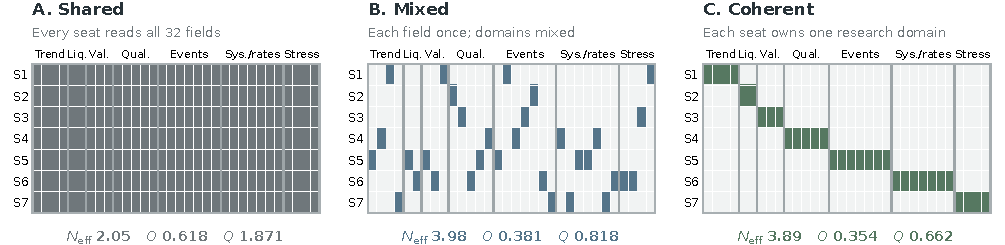
\includegraphics[width=0.94\textwidth]{fig_design_cropped}
\captionsetup{width=0.94\textwidth}
\caption{Bundled information-access treatment. Rows are seats and columns are the same 32 point-in-time fields; a filled cell grants a seat access to a field. Shared access broadcasts all fields, while mixed and coherent splits assign each once with the same packet-size profile. Coherent access preserves seven economic research domains. Values are 34-date means at $K=7$.}
\Description{Three access matrices compare shared access, mixed splitting, and coherent splitting. Shared access is full, mixed access is scattered, and coherent access forms research-domain blocks.}
\label{fig:design}
\end{figure*}

At seven seats, shared access yields \SharedKSeven\ effective books, versus \MixedKSeven\ and \CoherentKSeven; the assignment-averaged mixed gain is positive at all 34 month-ends and averages \MixedSharedNeff\ (95\% three-month moving-block bootstrap interval: \MixedSharedNeffCI). Coherent domains preserve similar breadth while reducing same-side overlap, demand in proposed books, and order concentration. The shared-versus-split contrast also appears in three markets and a long-only sensitivity.

Specifically, our contributions are the following:
\begin{itemize}[leftmargin=1.55em,itemsep=1.5pt,topsep=2pt,parsep=0pt]
\item We formulate inference-time information access as a team-design variable and test a bundled treatment of packet scope and assignment while holding the roster, prompt, mandate, team-level evidence, and aggregation rule fixed.
\item We introduce the Effective-Book Curve and order diagnostics for independent position directions, same-side overlap, internally netted gross, and liquidity-scaled order concentration. These measures capture portfolio dependence that answer-level diversity and single-model performance do not.
\item Across U.S. equities, European equities, crypto perpetuals, repeated generation, risk-space measurement, and a long-only sensitivity, we document shared-versus-split differences in measured breadth and demand in proposed books. A separate within-route diagnostic measures split-book breadth without a matched shared control.
\end{itemize}

\section{Related Work}
Our study connects financial LLM decisions, diversity in model teams, and dependence among funded portfolios. We focus on evidence organization before outputs are aggregated or capitalized.

\subsection{Financial LLM decisions and agent teams}
Financial LLM research shows that model outputs can contain return-relevant information while also inheriting systematic confirmation and portfolio biases~\cite{lopezlira2023chatgpt,lee2025yourai,winder2025biasedechoes}. Related systems translate text into allocations, construct multi-model portfolios from shared public information, or use synthetic personas to produce heterogeneous views~\cite{oh2025democratizing,iadisernia2025prompting}. Multi-agent trading frameworks assign technical, fundamental, news, and risk functions, while market simulations evaluate returns and aggregate dynamics~\cite{xiao2024tradingagents,miyazaki2026expertteams,wang2026macroeconomists,lopezlira2025market}.

These studies examine decision usefulness and coordinated specialization, but their components often vary together, so they do not isolate independence due to model identity, evidence access, communication, or aggregation. We fix the roster, mandate, prompt, team-level evidence, and output rule, vary the bundled field allocation, and retain every book before aggregation. We measure observed breadth under this organization.

\subsection{Diversity through models and evidence}
Ensemble methods vary samples, features, or internal randomization and ask whether lower error dependence improves aggregate prediction~\cite{brown2005diversity,ho1998random}. Nominal plurality likewise need not imply effective diversity in LLM teams. Model families can exhibit correlated errors, and multi-agent scaling gains depend on how diversity interacts with coordination and compute~\cite{kim2025correlated,yang2026agentscaling,wunderlich2026pareto}.

Li et al.~\cite{li2026diverseevidence} study binary-event forecasting with a fixed evidence pool, partitioned into shared public and disjoint private subsets. Their InfoDelphi framework exchanges rationales during deliberation and combines final forecasts by confidence-weighted logit pooling; its outcomes are aggregate forecast accuracy and Brier score. They also evaluate a no-deliberation variant, so fixed evidence and independent outputs are not novel by themselves. Yang et al.~\cite{yang2026agentscaling} explain diminishing returns from correlated agent outputs through effective information channels and evaluate voting and debate systems. Their label-free proxy $K^*$ is the entropy effective rank of a Gram matrix of output embeddings, measuring semantic diversity rather than portfolio positions.

We share the principle that nominal agent count need not equal effective diversity, but target a different estimand. With the requested model roster, mandate, output rule, and team-level point-in-time evidence union fixed, we vary field access and retain each continuous signed book before communication or aggregation. We measure dependence through the cross-sectional book-correlation spectrum, using participation-ratio effective dimension, and complement it with same-side overlap and the proposed order footprint after internal netting. The contrast is therefore access-induced breadth of unaggregated positions, not deliberation gains, aggregate forecast quality, or semantic diversity: different reasoning can induce the same trade, while opposite books share a risk direction yet offset proposed demand.


\subsection{Portfolio breadth, crowding, and research capacity}
Portfolio research relates diversification to independent risk directions, benchmark-relative distinctiveness, and independent decisions~\cite{meucci2009enb,cremers2009activeshare,grinold2000active}. Common positions can generate shared liquidity demand, correlated deleveraging, and endogenous co-movement~\cite{khandani2011quants,bucci2020coimpact,lou2022comomentum}. These results explain why repeated views should not receive repeated capital.

We locate dependence at the mapping from an information-access matrix to proposed books, before funding or execution. Effective-book count measures spectral breadth, while overlap and order diagnostics distinguish offsetting disagreement from repeated proposed demand. This treats access as a portfolio-design variable linked to measured pre-allocation breadth.

\section{Information-Access Architecture}\label{sec:architecture}
\subsection{Problem statement}
We consider a team of $K$ research seats that allocates across $D$ assets at decision date $t$. The team observes a point-in-time evidence vector $x_t$ containing $F$ fields. Seat $i$ uses model route $m_i$, a common prompt $P$, and an access row $A_i\in\{0,1\}^{F}$. The complete architecture is the binary matrix $A\in\{0,1\}^{K\times F}$. Each model returns asset scores $s_{i,t}$, converted into a unit-gross, dollar-neutral active book:
\begin{align}
s_{i,t}&=\mathcal{M}_{m_i}(P,x_t\odot A_i),\\
w_{i,t}&=\frac{s_{i,t}-\bar{s}_{i,t}\mathbf{1}}
{\lVert s_{i,t}-\bar{s}_{i,t}\mathbf{1}\rVert_1}.\label{eq:bookmap}
\end{align}

The mapping from scores to weights, the mandate, and all parsing rules are identical across conditions. Section~\ref{sec:longonly} repeats the $K=7$ comparison with fully invested nonnegative portfolios.

The objective is not to maximize disagreement. It is to measure how many distinct proposed position directions appear when the same team-level evidence is organized differently. Investment quality, compliance, and model validation would be prior eligibility gates in deployment, but this experiment does not apply those gates. The metrics therefore measure geometric breadth, not quality-adjusted or fundable capacity.

\subsection{Access designs}
The treatment has three endpoints:
\begin{enumerate}[leftmargin=1.8em,label=\textbf{A\arabic*.},itemsep=2pt,topsep=2pt,parsep=0pt]
\item \textbf{Shared access.} Every seat receives the complete 32-field packet, so $A_{if}=1$ for every seat $i$ and field $f$.
\item \textbf{Mixed split.} Each field is assigned once, so $\sum_i A_{if}=1$, and packets deliberately combine fields from different research domains.
\item \textbf{Coherent split.} Each field is assigned once, while economically related fields remain together in research domains.
\end{enumerate}

The coherent hierarchy is nested as team size grows. At $K=2$, one seat covers market and risk evidence and the other covers company and event evidence. These desks divide progressively. At $K=7$, the domains are trend, liquidity, valuation, company quality, corporate events, systematic risk and rates, and idiosyncratic and stress risk. Every seat receives at least one asset-specific field from which to form a cross-sectional book.

Mixed packets use the same packet-size profile at every $K$. For $K=7$, we select the size-matched partition with the lowest fine-domain normalized mutual information among 100,000 seeded candidates, thereby defining the opposite endpoint to coherent organization. Both matrices and their hashes were frozen before final model collection. The prompt describes every input as a ``research packet'' and never names the condition or assigns a specialist identity. Seats respond independently before any communication or aggregation.

For $K\geq2$, we average every model subset and packet-to-model permutation within date. At $K=7$, each split design contains 5,040 assignments formed from 49 cached books. Every route occupies every packet equally often, removing route identity from the packet comparison. Reuse across assignments does not create additional observations because inference remains at the date level.

\subsection{Effective-book capacity}
Equation~\eqref{eq:bookmap} implies $\mathbf{1}^{\prime}w_{i,t}=0$ and $\lVert w_{i,t}\rVert_1=1$, so every output is a dollar-neutral, unit-gross active book. Because its cross-sectional mean is zero, Pearson correlation across assets equals cosine similarity. Define $u_{i,t}=w_{i,t}/\lVert w_{i,t}\rVert_2$ and $U_t=[u_{1,t},\ldots,u_{K,t}]$. The book-correlation matrix is therefore the Gram matrix $C_K=U_t^{\prime}U_t$. It is positive semidefinite, has unit diagonal, and satisfies $\operatorname{tr}(C_K)=K$.

Let $\lambda_1,\ldots,\lambda_K$ be the eigenvalues of $C_K$. Since $\lVert C_K\rVert_F^2=\operatorname{tr}(C_K^2)=\sum_{\ell}\lambda_\ell^2$, the participation-ratio effective dimension~\cite{mazzucato2016dimensionality} is
\begin{align}
N_{\mathrm{eff}}(K)
&=\frac{\operatorname{tr}(C_K)^2}{\lVert C_K\rVert_F^2}
 =\frac{(\sum_{\ell}\lambda_\ell)^2}{\sum_{\ell}\lambda_\ell^2}\\
&=\frac{1}{\sum_{\ell}p_\ell^2},
\qquad p_\ell=\lambda_\ell/K.\label{eq:neff}
\end{align}

Thus, $N_{\mathrm{eff}}$ is the inverse concentration of portfolio variation across orthogonal book directions. It equals one when all spectral mass lies in one direction and reaches $K$ when mass is uniform across $K$ orthogonal directions. More generally,
$1\leq N_{\mathrm{eff}}(K)\leq\operatorname{rank}(C_K)\leq\min\{K,D-1\}$,
where the last bound follows because dollar-neutral books lie in the subspace orthogonal to $\mathbf{1}$. The path from one to seven seats is the \emph{Effective-Book Curve}. It measures breadth rather than investment quality.

Writing $\rho_{ij}$ for book correlation and defining
$\kappa_K=2[K(K-1)]^{-1}\sum_{i<j}\rho_{ij}^2$, the unit diagonal gives
\begin{align}
\lVert C_K\rVert_F^2
&=K+2\sum_{i<j}\rho_{ij}^2
 =K\{1+(K-1)\kappa_K\},\\
N_{\mathrm{eff}}(K)
&=\frac{K}{1+(K-1)\kappa_K}.\label{eq:identity}
\end{align}

Capacity therefore decreases monotonically with squared cross-seat dependence. Coincident or exactly opposite books have $\kappa_K=1$ and one geometric direction, while orthogonal books have $\kappa_K=0$ and $K$ directions. Equation~\eqref{eq:identity} holds within each date and assignment; reported values average date-level transformed $N_{\mathrm{eff}}$ and are not computed from an average $\kappa_K$. The order diagnostics distinguish repeated same-side demand from internally offsetting dependence.

The dimension-matched reference follows from the same geometry. Mean-centering an isotropic random score leaves a direction that is uniform on the unit sphere in the $(D-1)$-dimensional dollar-neutral subspace. Rotational symmetry gives
$\mathbb{E}[(u_i^{\prime}u_j)^2]=1/(D-1)$ for independent books. Substitution into Equation~\eqref{eq:identity} yields the moment-matched reference
\begin{equation}
N_{\mathrm{null}}(K,D)\approx\frac{K}{1+(K-1)/(D-1)}.
\end{equation}
At $D=14$ and $K=7$, this value is \AnalyticNullKSeven. Because the expectation of a ratio need not equal the ratio of expectations, we also draw 10,000 standard-normal $D\times K$ score matrices, mean-center each book, and rescale gross exposure to one. The simulated mean is \NullKSeven\ with a 95\% range of \NullKSevenLow\ to \NullKSevenHigh. This benchmark controls for asset dimension and team size.

Different stock weights can still load the same market and sector risks. We therefore form a second correlation matrix using the point-in-time covariance estimate $\Sigma_t$ from the 252 daily log returns available at date $t$:
\begin{equation}
C^{\mathrm{risk}}_{ij,t}=\frac{w_{i,t}^{\prime}\Sigma_t w_{j,t}}
{\sqrt{(w_{i,t}^{\prime}\Sigma_t w_{i,t})(w_{j,t}^{\prime}\Sigma_t w_{j,t})}}.
\label{eq:riskcorr}
\end{equation}
Applying Equation~\eqref{eq:neff} to this matrix yields effective ex ante risk directions. No future return enters $\Sigma_t$, and we also evaluate 25\% and 50\% diagonal shrinkage.

\subsection{Order diagnostics}
Correlation treats a book and its exact opposite as equally dependent. To distinguish opposition from repeated demand, we define same-side overlap for unit-gross books $i$ and $j$ as
\begin{equation}
O_{ij}=\sum_a \min(|w_{ia}|,|w_{ja}|)
\mathbf{1}\!\left\{\operatorname{sign}(w_{ia})=\operatorname{sign}(w_{ja})\right\}.
\label{eq:overlap}
\end{equation}
Zero denotes no same-side overlap and one denotes complete overlap. We average $O_{ij}$ across seat pairs and assignments within date.

We also translate the books into two intended-order measures, using each asset's average daily dollar volume (ADV):
\begin{equation}
\begin{aligned}
G&=\frac{\sum_a |\sum_i w_{ia}|}{\sum_i\sum_a |w_{ia}|}, &
Q&=\frac{\sum_a |\sum_i w_{ia}|^{3/2}/\mathrm{ADV}_a^{1/2}}
{\sum_i\sum_a |w_{ia}|^{3/2}/\mathrm{ADV}_a^{1/2}}.
\end{aligned}
\label{eq:orders}
\end{equation}
$G$ is the gross exposure remaining after internal netting, so $100G$ is external gross in millions for \$100 million of equal seat budgets. The dollar amount is a linear reporting normalization, not an estimate of deployable capital or market capacity. $Q$ compares combined orders with separate orders under an ADV-scaled square-root convention~\cite{bucci2020coimpact}. Common-book correlation additionally averages each seat's correlation with the mean of the other seats. These measures describe proposed demand and do not assume realized price impact.

The main reported contrast is mixed minus shared $N_{\mathrm{eff}}$ at $K=7$, with 100,000 overlapping, noncircular three-month moving-block draws after within-date averaging~\cite{kunsch1989bootstrap}. We report the 2.5th and 97.5th percentiles as 95\% intervals. The target and inference population are date-level means; six-month blocks give the same interpretation. All other results and intervals are secondary or exploratory, pointwise, and unadjusted for multiplicity; repeat and cross-market panels resample dates. Exclusion of zero in these secondary intervals is not a familywise-controlled significance claim.

\subsection{Connections to ensemble and portfolio design}
The access treatment shares a design principle with feature-based ensemble diversity, but it operates at a different stage of the learning system. Random-subspace and related methods train or fit predictors on different feature sets and evaluate the accuracy of their aggregate~\cite{brown2005diversity,ho1998random}. Here the requested model routes are fixed, the intervention occurs at inference time, and the complete point-in-time evidence set remains available to the team. The object of study is therefore the organization of research rather than the estimation of model parameters.

This distinction changes the relevant outcome. Prediction accuracy alone does not translate into distinct capital opportunities when different forecasts induce the same trade. Repeated same-side positions consume one liquidity channel, while opposite positions can be highly correlated in geometry yet internally net before reaching the market. Effective dimension and order diagnostics are therefore complementary. $N_{\mathrm{eff}}$ records the number of active-risk directions in the eigenvalue spectrum of the book-correlation matrix, and $O$, $G$, and $Q$ determine whether those directions reproduce or offset demand.

The Effective-Book Curve is a team-size frontier of geometric breadth, not of quality-adjusted funding opportunities. At each $K$, the split architecture is rebalanced according to the same mixed or coherent design rule. The curve therefore compares complete $K$-seat organizations rather than appending one fixed packet to an otherwise unchanged team. Its slope shows how efficiently an architecture converts nominal research seats into distinct proposed directions. Access architecture sits between model selection and capital allocation; the curve alone does not determine which directions an allocator should fund.

\section{Experimental Protocol}\label{sec:protocol}
We evaluate the access architecture through a pooled U.S. panel and a set of transfer tests. Section~\ref{sec:primaryprotocol} describes the point-in-time data, model collection, and assignment protocol. Section~\ref{sec:transferprotocol} summarizes repeated generation, cross-market transfer, and long-only mandate transfer.

\subsection{Pooled U.S. panel}\label{sec:primaryprotocol}
The pooled U.S. experiment uses 34 month-ends from July 2023 through April 2026 and 14 liquid U.S. large-cap stocks across seven sectors: AAPL, MSFT, NVDA, GOOGL, META, AMZN, TSLA, WMT, PG, JPM, BAC, XOM, JNJ, and UNH. The universe was fixed before final collection; the same seven-route roster and model-vintage window apply in every condition. Twelve dates informed design development, 22 form a complementary, non-confirmatory sensitivity, and all 34 comprise the pooled U.S. panel.

The 32 fields span seven research domains. Trend uses 5-, 21-, and 63-session returns and drawdown; the historical return labels are 7d, 30d, and 90d. Liquidity uses volatility and average daily dollar volume. Valuation uses price-to-earnings, price-to-sales, and price-to-book ratios. Company quality covers profitability, leverage, cash, growth, and reporting history. Corporate events summarize recent 8-K, earnings, and material-event activity. The final domains combine asset sensitivities with rates and stress indicators. Observation and filing cutoffs exclude dates after the decision date, and forward returns never enter a prompt. Prices and market series come from Yahoo Finance, and accounting and filings from SEC EDGAR. Valuation prices and share counts are split-adjusted to a July 20, 2026 corporate-action cutoff, while return, volatility, drawdown, and beta fields use an adjusted-close series; neither is a historical download-vintage archive. Source URLs, cutoffs, and hashes accompany the frozen packets.

A route is a requested OpenRouter model endpoint; the recorded routed provider is its realized backend. A seat pairs one route with one packet, and its structured portfolio output is a book. Registration is the \texttt{created} timestamp in the July 21, 2026 OpenRouter catalog snapshot; cutoff is the latest registration in the sensitivity. Eligibility gates are investment quality, compliance, and model validation, which the experiment does not evaluate. ``Prespecified'' applies only to access-design elements frozen before final model collection.

The requested routes are \path{openai/gpt-4o}, \path{google/gemini-2.5-flash}, \path{meta-llama/llama-3.1-70b-instruct}, \path{qwen/qwen3-235b-a22b-2507}, \path{mistralai/mistral-large}, \path{deepseek/deepseek-chat}, and \path{anthropic/claude-sonnet-4.5}. These identify requested endpoints, not immutable model weights; serving providers can vary. U.S. responses were collected at temperature 0.7 with a common prompt that hides the calendar date and forbids outside facts or inference about missing fields. Structured output covers all 14 assets and must form a nonzero active book. We retain generation IDs, routed providers, requested models, prompt and packet hashes, and seed metadata, including recorded recovery offsets.

\begin{table}[!t]
\caption{The pooled U.S. protocol holds the research problem fixed.}
\label{tab:protocol}
\centering
\footnotesize
\begin{tabular*}{\linewidth}{@{\extracolsep{\fill}}ll}
\toprule
Design item & Frozen specification \\
\midrule\addlinespace[2.5pt]
Primary sample & U.S. equities · 34 month-ends · 14 assets \\
Team & 7 model routes · research seats K=1 to K=7 \\
Fixed evidence & 32 point-in-time fields · same union in every condition \\
Access conditions & shared access · mixed split · coherent split \\
Inference unit & date · all model/packet assignments averaged within date \\
\bottomrule
\end{tabular*}

\tabnote{The 32 fields enter each split team exactly once. Shared access duplicates the same union across seats. Prompt fields are timestamped at the decision date, and inference is conducted at the date level.}
\end{table}

The pooled U.S. collection contains 13,090 archived books. Deterministic scripts regenerate every reported quantity from frozen packets, access matrices, request metadata, and model responses.

\paragraph{Executed-protocol record.}
The accompanying reproducibility record supplies requested and canonical route identifiers, observed providers, both frozen $7\times32$ access matrices, all 32 field definitions and transformations, and the full executed prompt and application programming interface (API) output schema. Machine-readable protocol, schema, template, and rendered examples are available in the public repository. The record distinguishes API-schema constraints from collector checks and prompt-only instructions.

\subsection{Robustness and transfer panels}\label{sec:transferprotocol}
The repeatability panel probes whether the access comparisons persist across stochastic generation. Six frozen dates span three return and two volatility regimes. Seven routes are evaluated under shared-full, shared-small, mixed, and coherent conditions at temperatures 0.0 and 0.7, with three calls per route-packet cell. Shared-small broadcasts one short packet, and a common complete-block rule retains 35 of 36 replicate blocks. This six-date repeat check is distinct from the 34-date broadcast control.

The harmonized cross-market panel covers 12 common dates in U.S. equities, European equities, and crypto perpetuals. Each market uses the same 32 timestamped price-volume fields for trend, reversal, volatility, tail risk, systematic exposure, liquidity, and cross-sectional ranks. Each equity universe contains 14 liquid stocks, and the crypto universe contains 12 liquid perpetuals. Routes, prompt, portfolio rule, fields, and assignment algorithm are identical. All comparisons are made within market.

For the long-only transfer, the seven routes produce fully invested nonnegative portfolios on the 34 U.S. dates using the pooled U.S. panel's same 32 fields and frozen pooled-panel $K=7$ assignments. Active weights are $a_i=p_i-1/14$ and are rescaled to unit gross for seat-level diagnostics. The team averages the seven seats equally. Model-to-packet assignments remain fixed across 34 nonoverlapping monthly windows, with signals entering at the first close after month-end and exiting at the next month-end close. Split results average 5,040 fixed assignment paths and report gross returns.

The LLM routes are experimental subjects. OpenAI Codex assisted with implementing and debugging analysis code, checking reported quantities against frozen outputs, and preparing deterministic figure scripts. The authors reviewed the code and outputs and made all design and interpretation decisions.

\section{Experiments}\label{sec:experiments}
We first trace how measured capacity scales with team size. We then report diagnostics for within-route behavior, packet broadcast, repeated generation, and risk-space measurement. Finally, we examine proposed-order outcomes, cross-market transfer, and long-only portfolios.

\subsection{The Effective-Book Curve}
Figure~\ref{fig:curve} shows that shared access adds responses faster than position directions. The curve reaches \SharedKTwo\ effective books at two seats, \SharedKFour\ at four, and \SharedKSeven\ at seven. Shared-access marginal capacity falls at every step. The second seat adds \SharedFirstMarginal\ of an effective book, while the seventh adds \SharedLastMarginal.

\begin{figure}[!t]
\centering
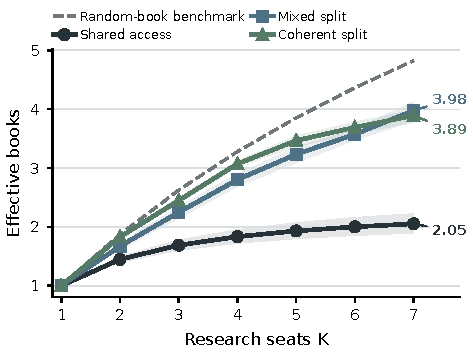
\includegraphics[width=\columnwidth]{fig_capacity_curve}
\caption{Information access shifts the Effective-Book Curve in the pooled U.S. panel. Lines are 34-date means and bands are three-month moving-block 95\% intervals. The dashed line is the dimension-matched random-book benchmark. $K=1$ is the common one-seat starting point.}
\Description{Shared access bends toward two effective books. Mixed and coherent splits move the curve upward as team size grows.}
\label{fig:curve}
\end{figure}

At $K=7$, shared access reaches \SharedNullShare\ of the \NullKSeven-book random reference. Mean squared off-diagonal correlation is \SharedKappa, versus \MixedKappa\ and \CoherentKappa; the analytic random reference is \NullKappa. By Equation~\eqref{eq:identity}, shared seats retain a common loading while split seats recover substantial breadth. Mixed reaches \MixedKSeven, or \MixedNullShare\ of the random-book mean, marginally below the simulated distribution's 2.5th percentile of \NullKSevenLow; this proximity establishes neither predictive quality nor noise equivalence.

The coherent curve rises faster at small and intermediate team sizes and ends at \CoherentKSeven; mixed ends slightly higher at $K=7$. This pooled-panel mixed-over-coherent ordering reverses in the harmonized panel, where coherent exceeds mixed while both splits exceed shared. Different field universes may explain this contrast, but the experiment does not identify its cause or establish a universal mixed-versus-coherent ranking.

\begin{table}[!t]
\caption{Split access nearly doubles measured effective-book breadth and reduces overlap in proposed orders.}
\label{tab:primary}
\centering
\footnotesize
\begin{tabular*}{\linewidth}{@{\extracolsep{\fill}}lccc}
\toprule
Outcome / check & Shared & Mixed & Coherent \\
\midrule\addlinespace[2.5pt]
Effective books (higher) & 2.05 & 3.98 & 3.89 \\
Same-side overlap (lower) & 0.618 & 0.381 & 0.354 \\
Proposed external gross from \$100M (lower) & \$79.0M & \$45.7M & \$41.3M \\
Order concentration (lower) & 1.871 & 0.818 & 0.662 \\
Common-book correlation & 0.725 & 0.215 & 0.147 \\
Complementary 22 dates: effective books & 2.00 & 3.98 & 3.87 \\
Within-route split check & N/A & 3.81 & 3.56 \\
Repeat check: effective books (6 dates) & 1.84 & 4.24 & 3.70 \\
Risk-space check (random ref. 3.81) & 1.79 & 2.73 & 2.59 \\
\bottomrule
\end{tabular*}

\tabnote{The first five rows are 34-date means at $K=7$. The complementary row uses 22 dates not used in development and is non-confirmatory. The within-route row has no matched shared baseline; the repeat row averages three $T=0.7$ calls over six dates, and the risk row uses trailing 252-day returns. Proposed external gross is $100G$ million under a \$100 million normalization, not measured deployable capacity.}
\end{table}

\subsection{Within-route diagnostic}
Seven mixed packets through one fixed route yield \WithinRouteMixedNeff\ effective books, versus \MixedKSeven\ across seven routes; coherent counts are \WithinRouteCoherentNeff\ and \CoherentKSeven. These are descriptive breadth levels for split access. Without a matched within-route shared baseline, it identifies neither a within-route access effect nor route diversity's contribution.

\subsection{Date and assignment sensitivity}
For the seven-route teams at $K=7$, mixed raises assignment-averaged breadth from \SharedKSeven\ to \MixedKSeven, a paired gain of \MixedSharedNeff\ (95\% interval: \MixedSharedNeffCI), positive on all 34 dates. Figure~\ref{fig:time} compares these same-date means; it does not assert that every individual assignment outperforms shared access.

\begin{figure}[!t]
\centering
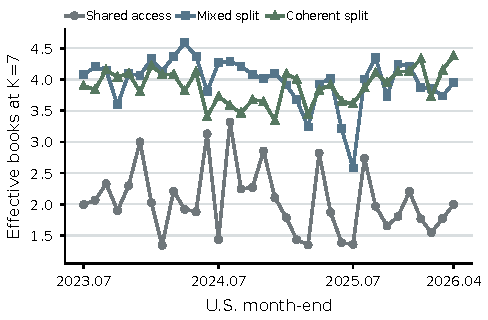
\includegraphics[width=\columnwidth]{fig_capacity_time}
\caption{Same-date, assignment-averaged $K=7$ breadth across 34 U.S. month-ends. The minimum-to-maximum ranges across dates are \SharedNeffRange\ for shared, \MixedNeffRange\ for mixed, and \CoherentNeffRange\ for coherent access. Those marginal time ranges can overlap even though the split-minus-shared gap is positive at every matched date. Each point averages all valid model-to-packet assignments within date.}
\Description{A monthly line chart shows that both split-access designs have more effective books than shared access at every U.S. month-end, although all three levels vary over time.}
\label{fig:time}
\end{figure}

The 22 dates not used in development are a complementary, non-confirmatory sensitivity: mixed and coherent gains are \ComplementMixedGain\ and \ComplementCoherentGain, positive on all 22. All 34 dates comprise the pooled panel. On all eight month-ends after the latest recorded route registration, beginning \PostRegistrationStart, gains are \PostRegistrationMixedGain\ and \PostRegistrationCoherentGain. Mixed exceeds shared at every $K=2,\ldots,7$.

\paragraph{Assignment sensitivity.}
Across all 5,040 route-to-packet bijections within each date, mixed access has date-averaged within-date 5th, 50th, and 95th percentiles of \ADMixedNeffLow, \ADMixedNeffMedian, and \ADMixedNeffHigh\ effective books; coherent access has \ADCoherentNeffLow, \ADCoherentNeffMedian, and \ADCoherentNeffHigh. The mean within-date fraction exceeding the same-date shared team is \ADMixedAbovePercent\% and \ADCoherentAbovePercent\%, respectively. Some assignments fall below shared on \ADMixedNegativeDates\ and \ADCoherentNegativeDates\ of the 34 dates. Positive assignment-averaged gains therefore do not imply uniform assignment-level dominance. These are descriptive within-date quantiles averaged across dates, not pooled quantiles or confidence intervals; inference remains date-level.

Three secondary or exploratory checks preserve the reported access comparisons. First, the 34-date broadcast control yields \ShortMixedBroadcastNeff\ to \ShortCoherentBroadcastNeff\ effective books across packet sets, versus \MixedKSeven\ and \CoherentKSeven\ when packets differ. Second, in six-date repeats, shared yields \RepeatSharedTZero\ to \RepeatSharedTSeven\ and mixed \RepeatMixedTZero\ to \RepeatMixedTSeven, with positive paired gaps on all dates. The persistent shared-small condition averages \RepeatSmallTZero\ at 0.0 and \RepeatSmallTSeven\ at 0.7, reaches \RepeatSmallException\ on one date, and mixed remains \RepeatMixedExceptionRange\ there. Third, risk-space counts are \RiskSharedNeff, \RiskMixedNeff, and \RiskCoherentNeff\ against \RiskNullNeff; mixed reaches \RiskMixedNullShare, exceeds shared on \RiskMixedPositiveDates\ of 34 dates, and has a gain of \RiskMixedSharedNeff\ (\RiskMixedSharedNeffCI). The ordering also survives 25\% and 50\% shrinkage.

\subsection{Operational consequences and cross-market transfer}
Effective-book count records independent directions, while order diagnostics distinguish whether those directions coincide in proposed demand. Relative to shared access, mixed lowers same-side overlap from \SharedOverlap\ to \MixedOverlap, proposed external gross from \$79.0 million to \$45.7 million for \$100 million of equal seat budgets, order concentration from \SharedOrder\ to \MixedOrder, and common-book correlation from \SharedCommonBeta\ to \MixedCommonBeta.

\paragraph{Prompt usage and request cost.}
Mixed access uses \MixedPromptTokenReduction\ fewer prompt tokens (team means of 18{,}480 versus 5{,}944) and \MixedReportedCostReduction\ less model-reported request cost than shared access. These are archived usage and reported-cost measures, not evidence of lower end-to-end operating cost, latency, or improved investment quality.

For coherent minus mixed, the difference in overlap is $\CoherentMixedOverlap$ ($\CoherentMixedOverlapCI$), the difference in proposed external gross is $\CoherentMixedGross$ ($\CoherentMixedGrossCI$), and the difference in order concentration is $\CoherentMixedOrder$ ($\CoherentMixedOrderCI$). These exploratory, pointwise intervals exclude zero without multiplicity correction; they describe the pooled-panel tendency toward less same-side demand under coherent access, not a universally superior design.

\begin{figure}[!t]
\centering
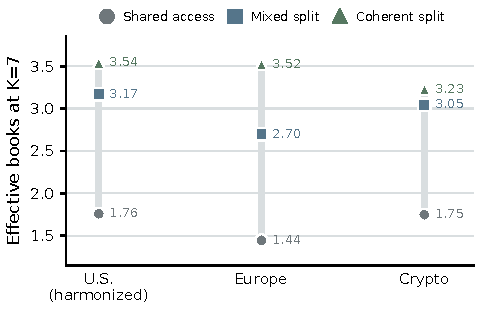
\includegraphics[width=\columnwidth]{fig_crossmarket}
\caption{The shared-versus-split ordering repeats in the harmonized 12-date panel. Each market uses the same market-risk field definitions, seven routes, prompt template, parser, and portfolio rule. The U.S. label refers to the harmonized panel, while the pooled U.S. panel also uses fundamentals and filings. Labels are date means at $K=7$.}
\Description{Shared access produces the fewest effective books in U.S. equities, European equities, and crypto perpetuals. Mixed and coherent splitting raise the count.}
\label{fig:crossmarket}
\end{figure}

In harmonized U.S. equities, European equities, and crypto perpetuals, both splits exceed shared, and coherent exceeds mixed, reversing the pooled U.S. order. Europe moves from \CrossEUSharedNeff\ to \CrossEUCoherentNeff, and crypto from \CrossCryptoSharedNeff\ to \CrossCryptoCoherentNeff. The secondary mixed-minus-shared intervals exclude zero in all markets under the convention above. Low-retry three-route gains are \CrossUSStableMixedGain, \CrossEUStableMixedGain, and \CrossCryptoStableMixedGain; all-route $K=3$ gains are \CrossUSKThreeMixedGain, \CrossEUKThreeMixedGain, and \CrossCryptoKThreeMixedGain. These track the full roster despite retry rates \CrossUSRetryRate, \CrossEURetryRate, and \CrossCryptoRetryRate. They describe harmonized-protocol transfer, not a mechanism or quality attribution.

\begin{table}[!t]
\caption{Coherent access reduces overlap in proposed orders across all three markets.}
\label{tab:markets}
\centering
\footnotesize
\begin{tabular*}{\linewidth}{@{\extracolsep{\fill}}lccc}
\toprule
Market & Overlap $O$ & Proposed external gross (\$M) & Concentration $Q$ \\
\midrule\addlinespace[2.5pt]
U.S. & 0.659 → 0.367 & 84.5 → 45.0 & 2.089 → 0.797 \\
Europe & 0.720 → 0.353 & 89.8 → 42.2 & 2.274 → 0.749 \\
Crypto & 0.670 → 0.404 & 84.9 → 49.8 & 2.172 → 0.958 \\
\bottomrule
\end{tabular*}

\tabnote{Entries are 12-date means at $K=7$, with arrows running from shared to coherent access. $O$ is same-side overlap, $100G$ is proposed external gross in millions for equal seat budgets summing to \$100 million, and $Q$ is ADV-scaled order concentration. Lower values indicate less same-side overlap, external gross, or order concentration, respectively.}
\end{table}

For \$100 million of equal seat budgets, coherent lowers proposed external gross from \$84.5 million to \$45.0 million in the United States, \$89.8 million to \$42.2 million in Europe, and \$84.9 million to \$49.8 million in crypto. In each harmonized panel, lower demand in the proposed books accompanies greater measured breadth than under shared access.

\subsection{Long-only mandate transfer}\label{sec:longonly}
We report a long-only sensitivity under a fully invested institutional mandate. Shared access remains the experimental control, while equal weight provides a passive within-universe reference.

\begin{figure*}[!t]
\centering
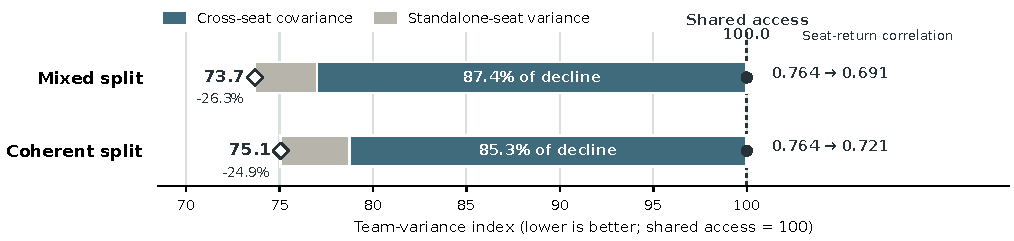
\includegraphics[width=0.92\textwidth]{fig_allocation_decomposition}
\captionsetup{width=0.92\textwidth}
\caption{Long-only team-variance decomposition. Shared access is normalized to 100. Each bar runs from the split outcome to that benchmark and decomposes the observed decline into lower standalone-seat variance and lower cross-seat covariance over the same 34 monthly windows. Split designs average 5,040 fixed model-to-packet paths.}
\Description{Horizontal bars run from each split design's normalized team variance to the shared-access benchmark of 100, with segments for standalone-seat variance and cross-seat covariance.}
\label{fig:allocation-decomposition}
\end{figure*}

\begin{table}[!t]
\caption{Descriptive long-only gross-return sensitivity.}
\label{tab:longonly}
\centering
\footnotesize
\begin{tabular*}{\linewidth}{@{\extracolsep{\fill}}lcccc}
\toprule
Portfolio outcome & Equal wt. & Shared & Mixed & Coherent \\
\midrule\addlinespace[2.5pt]
Effective active books & N/A & 2.41 & 3.73 & 3.68 \\
Active same-side overlap & N/A & 0.562 & 0.404 & 0.378 \\
Effective holdings & 14.0 & 8.4 & 11.3 & 11.8 \\
Top-three weight & 21.4\% & 49.2\% & 36.9\% & 34.8\% \\
Largest stock weight & 7.1\% & 21.0\% & 14.8\% & 14.0\% \\
Annualized return & 24.38\% & 27.49\% & 26.28\% & 26.09\% \\
Annualized volatility & 13.03\% & 15.94\% & 13.67\% & 13.80\% \\
Drawdown magnitude & 9.08\% & 16.57\% & 10.18\% & 9.46\% \\
Sharpe ratio & 1.526 & 1.442 & 1.594 & 1.566 \\
Monthly rebalance turnover & 2.6\% & 31.2\% & 17.1\% & 14.0\% \\
\bottomrule
\end{tabular*}

\tabnote{Entries use 34 nonoverlapping monthly windows at $K=7$. Shared is the fixed seven-route experimental control; equal weight is a passive reference holding the same 14 stocks at $1/14$. Split diagnostics average 5,040 assignments within date, and path statistics are then averaged across assignments. Returns are gross, not evidence of causal performance superiority. Sharpe subtracts the point-in-time three-month Treasury yield divided by 12.}
\end{table}

Shared access produces \LongSharedNeff\ effective active books, compared with \LongMixedNeff\ and \LongCoherentNeff\ under mixed and coherent access. Active overlap falls from \LongSharedOverlap\ to \LongMixedOverlap\ and \LongCoherentOverlap. Effective holdings rise from \LongSharedHoldings\ to \LongCoherentHoldings, while top-three weight declines from \LongSharedTopThree\% to \LongCoherentTopThree\%. Mixed minus shared is \LongMixedSharedNeff\ books ($\LongMixedSharedNeffCI$) and $\LongMixedSharedOverlap$ in overlap ($\LongMixedSharedOverlapCI$). Coherent minus shared is \LongCoherentSharedNeff\ books ($\LongCoherentSharedNeffCI$) and $\LongCoherentSharedOverlap$ in overlap ($\LongCoherentSharedOverlapCI$). Under the pointwise, unadjusted convention above, these secondary intervals exclude zero. Equal weight is a passive anchor rather than the treatment control. It holds \LongEqualWeightHoldings\ effective names, while the coherent team retains active tilts and spreads weight across \LongCoherentHoldings\ names.

Shared access earns \LongSharedReturn\% gross with \LongSharedVolatility\% volatility. Mixed and coherent access earn \LongMixedReturn\% and \LongCoherentReturn\%, with volatilities of \LongMixedVolatility\% and \LongCoherentVolatility\%. Their Sharpe ratios are \LongMixedSharpe\ and \LongCoherentSharpe, compared with \LongSharedSharpe\ for shared access and \LongEqualWeightSharpe\ for equal weight. Coherent access improves drawdown by \LongCoherentDrawdownImprovement\ percentage points and lowers monthly turnover from \LongSharedTurnover\% to \LongCoherentTurnover\%. On the same holding windows, mixed minus shared monthly return is $\LongMixedSharedMonthlyReturn$ percentage points ($\LongMixedSharedMonthlyReturnCI$), and coherent minus shared is $\LongCoherentSharedMonthlyReturn$ ($\LongCoherentSharedMonthlyReturnCI$). Both secondary return intervals include zero. At similar gross returns, this sensitivity reports more independent active books and lower concentration, risk, drawdown, and turnover under split access; it does not establish predictive quality, realized performance, or information-driven diversification rather than dilution toward equal weight.

Lower team volatility can arise from quieter sleeves or from less co-movement across sleeves. For access architecture $h$, equal seat budgets, and seat return $r_{i,t}^{h}$, define
\begin{align}
V_{\mathrm{team}}^{h}
&=\operatorname{Var}(\bar r_t^{h})
 =V_{\mathrm{seat}}^{h}+V_{\mathrm{cross}}^{h},\\
V_{\mathrm{seat}}^{h}
&=\frac{1}{K^2}\sum_i\operatorname{Var}(r_{i,t}^{h}),
\qquad
V_{\mathrm{cross}}^{h}
=\frac{2}{K^2}\sum_{i<j}\operatorname{Cov}(r_{i,t}^{h},r_{j,t}^{h}).
\label{eq:allocation-variance}
\end{align}
For split architecture $p$ relative to shared access $s$, the fraction of the team-variance decline attributable to lower cross-seat covariance is
\begin{equation}
\chi_{\mathrm{cross}}(p;s)=
\frac{V_{\mathrm{cross}}^{s}-V_{\mathrm{cross}}^{p}}
{V_{\mathrm{team}}^{s}-V_{\mathrm{team}}^{p}}.
\label{eq:covariance-share}
\end{equation}
Mean pairwise seat-return correlation falls from \AllocationSharedCorrelation\ under shared access to \AllocationMixedCorrelation\ under mixed and \AllocationCoherentCorrelation\ under coherent access. Team variance falls by \AllocationMixedVarianceReduction\ and \AllocationCoherentVarianceReduction. Equation~\eqref{eq:covariance-share} reports \AllocationMixedCovarianceShare\ and \AllocationCoherentCovarianceShare\ as the shares of those observed declines attributable to lower cross-seat covariance. Mixed delivers the larger observed covariance reduction, while coherent delivers lower position overlap, common-book correlation, and order concentration.

\subsection{Discussion}
\paragraph{What makes information access consequential?}
The bundled comparisons document three aspects of portfolio organization; they do not isolate the mechanism behind each difference.
\begin{enumerate}[leftmargin=1.7em,label=\textbf{\arabic*.},itemsep=2pt,topsep=2pt,parsep=0pt]
\item \textbf{Access changes the conditional research problem.} A model is not an independent analyst in isolation. Its book is conditional on the evidence it receives. Broadcasting the same packet preserves a common information state across model families, while split access creates distinct inference problems without changing the team's evidence union.
\item \textbf{Breadth and organization are separate design objectives.} Mixed access produces slightly larger position-space breadth at $K=7$ in the pooled U.S. panel, but coherent access leads in the harmonized panel. Coherent access also lowers overlap, proposed external gross, and order concentration in the tested comparisons. Neither architecture is universally superior, and greater breadth by itself is not a quality criterion.
\item \textbf{Long-only sensitivity is descriptive.} The long-only decomposition reports lower cross-seat co-movement as one component of the observed team-variance decline. Dilution toward equal weight remains an alternative explanation, so the result is descriptive rather than evidence of a predictive mechanism.
\end{enumerate}

\paragraph{Funding implication.}
These measures provide a pre-deployment diagnostic of breadth and demand in proposed books under the tested access allocations. Subject to separate quality, compliance, validation, and portfolio gates, a research process can preserve seat-level books and measure effective capacity, overlap, proposed external gross, order concentration, and common-book correlation before deployment. They do not establish fundability or realized execution effects.

\paragraph{Limitations.}
The pooled U.S. panel uses one 14-stock universe, one model-vintage window, and structured point-in-time packets. Europe and crypto test transfer under a harmonized market-data protocol, but broader universes and later vintages would sharpen external validity. Mixed and coherent access are bundled treatment endpoints rather than a distribution over all partitions, so the comparisons do not identify individual access, packet, or assignment mechanisms. A quality-adjusted frontier across many architectures is a natural next step.

The study measures independent-book breadth rather than standalone alpha. The long-only results are a descriptive sensitivity showing similar gross returns and lower risk and turnover; they do not separate information-driven diversification from dilution toward equal weight, and longer histories and ex ante quality scores are needed after a common performance threshold. Historical replay with visible tickers can affect return levels, although every condition shares routes, dates, and assets. The order measures describe proposed demand, and returns are gross. The study does not measure live orders, fills, implementation shortfall, deployable capacity, or realized impact.

\section{Conclusion}
We introduced the Effective-Book Curve to measure independent-book breadth in LLM investment teams. The central finding is that nominal model count and independent book count can diverge sharply. Seven routes reading one packet produce \SharedKSeven\ effective books, while assigning each field once produces approximately four. The within-route split diagnostic also shows substantial breadth, but its unmatched design identifies neither an access effect nor route diversity's contribution.

The result is not limited to one geometric metric. Split access lowers same-side overlap, proposed external gross, order concentration, and common-book correlation. Coherent research domains preserve nearly the same breadth as mixed packets while producing the smallest overlap in proposed orders. Both split designs exceed shared access in the harmonized U.S. equity, European equity, and crypto-perpetual panels, while coherent exceeds mixed there, reversing the pooled-panel ordering. The long-only sensitivity reports lower cross-seat covariance as a component of the observed team-variance reduction.

An LLM investment team can be evaluated as an information architecture, not only as a roster of models. Quality and compliance gates determine which views are eligible. The Effective-Book Curve then provides a pre-deployment diagnostic of distinct proposed directions and repeated demand under the tested allocation contrast. These quantities concern proposed books; they do not show that a direction is fundable or executable, or that a proposed order would be filled or have realized impact.

\section*{Disclaimer}
The views expressed are solely those of the authors and do not represent EY Consulting, Mirae Asset Securities, or DS Investment \& Securities. The authors are responsible for any errors or omissions. This paper is for academic purposes only and does not constitute investment advice, a recommendation, solicitation, or an offer to buy or sell financial products or securities.

\section*{Acknowledgements}
This research was supported by the Basic Science Research Program through the National Research
Foundation of Korea (NRF), funded by the Ministry of Education (RS-2026-25576625), and by an NRF
grant funded by the Korean government (MSIT) (RS-2023-00242528).

\bibliographystyle{ACM-Reference-Format}
\bibliography{\ReviewBibliography}

\end{document}
